\documentclass[conference]{IEEEtran}
\usepackage[backend=biber, citestyle=ieee]{biblatex}
\usepackage[T1]{fontenc}
\usepackage[utf8]{inputenc}
\usepackage{amsmath, amssymb, amsfonts}
\usepackage{algorithmic}
\usepackage{graphicx}
\usepackage{subcaption}
\usepackage{textcomp}
\usepackage{xcolor}
\usepackage{hyperref}
\usepackage{caption}
\captionsetup[figure]{font=small}
\addbibresource{main.bib}

\graphicspath{{imgs}}

\begin{document}
\title{Data Science Homework 5 Report}
\author{\IEEEauthorblockN{Andr\'es Ponce}
		\IEEEauthorblockA{\textit{Department of Computer Science and Information Engineering}}
		\textit{National Cheng Kung University}\\
		Tainan, Taiwan\\
		andresponce@ismp.csie.ncku.edu.tw
}
\maketitle
\begin{abstract}
	Facial verification is the task of taking two images and 
	deciding whether they are two images of the same faces.
	Many state-of-the-art approaches~\cite{yan2019vargfacenet}~\cite{Deng_2019_CVPR}~\cite{Shi_2019_ICCV}~\cite{boutros2019elastic}
	perform highly on datasets such as Labeled Faces in the Wild~\cite{LFWTech}.
	This report takes the ArcFace approach, and determines if a simpler backbone 
	architecture can perform about as well.
	Most papers on this subject employ the ResNet~\cite{he2016deep} architecture,
	but other, simpler architectures such as EfficientNet~\cite{tan2019efficientnet}
	can achieve similar performance.
	Alhtough we were not able to replicate the performance in the paper since we trained on
	different datasets, we show that both architectures perform about as well while 
	having different number of parameters.
	We train the different models first on the CASIA-WebFace dataset~\cite{casiawebface} then test
	on the LFW dataset and report the performance of different models.
	The code is available at \url{https://github.com/andrew15818/110/tree/master/spring/data_science/hw/hw5}.
\end{abstract}

\section{Introduction}
Convolutional Neural Networks (CNNs) are suited for many image-related tasks,
among those being face verification and face recognition.
Facial verification takes two images and predicts whether these belong to the same image.
This type of facial recognition is used by people many times every day when unlocking their phone,
or by confirming if different images contain the same person.
However, any model that deals with facial verification has to recognize the same person in different 
lighting conditions, angles, and with different facial expressions.

Although efficient facial detection has existed for many years, with algorithms such as 
Viola-Jones~\cite{viola2001rapid}, neural networks have allowed not only facial detection 
but also facial recognition and verification to become more commonplace.
These technologies are useful when authenticating a user or in other 
security applications.

In recent years there has also been a large growth in CNN models.
While some models are mostly concerned with the largest posible accuracy on a task,
many models are instead concerned with decreasing the number of parameters
and calculations necessary, possibly with slightly lower performance.

In this assignment, our aim was to test the ArcFace method and maintain 
similar performance while using a simpler architecture for face verificaiton.
In the following sections, we compare the ResNet architecture used~\cite{Deng_2019_CVPR}
with newer approaches such as EfficientNet.
Then, we discuss the experiments where use these two models to perform
face-verification.

\section{Model Comparison}
\begin{figure}[!t]
	\centering
	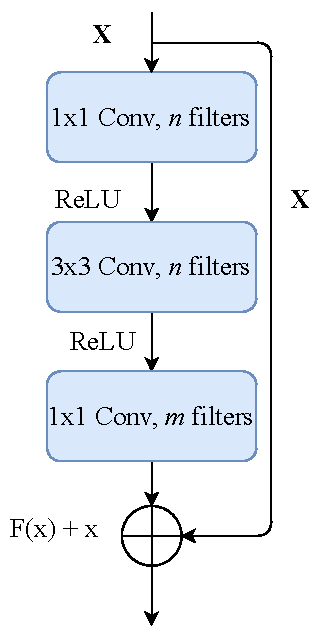
\includegraphics[scale=0.5]{resnet-block}
	\caption{Single ResNet block. The idea is for the block to learn 
	$\mathcal{H}(x)-x$, and at the end we add the original input (downsampled 
	so dimensions fit). 
	This is so that our model learns the residual $\mathcal{F}(x) = \mathcal{H}(x) + x$.}
	\label{fig:resnetblock}
\end{figure}
\subsection{ResNet}
The ResNet~\cite{he2016deep} architecture has become one of the most widely used
architectures in computer vision papers.
ResNets allowed deep networks to become much deeper by solving the vanishing gradient 
problem which had been a limiting factor in earlier models.
If a block normally learns the mapping $\mathcal{F}(\bold{x})$, the authors
instead have the model learn $\mathcal{H}(\bold{x}) - \boldsymbol{\bold{x}}$.
The output of the block then becomes $\mathcal{F}(\bold{x}) + \bold{x}$.
In the paper, they apply two convolutional operations separated by a ReLU activation
and add the original input $\bold{x}$ to the internal representation at the end.
The input $\bold{x}$ might also be downsampled so the dimensions match at the end of the block.

Stacking these residual blocks and changing the filters at each block result in some
of the variants such as ResNet18, ResNet50, ResNet101, and even ResNet152.
Fig~\ref{fig:resnetblock} shows a single block of ResNet50.
In the original paper, $m=4n$.
A certain number of blocks forms a group, each block having the same parameters.


\subsection{EfficientNet}
EfficientNet~\cite{tan2019efficientnet} models were developed to address the problem 
of scaling only one dimension when changing network parameters.
The authors look at three factors which control the dimensions of the network:
the ``width'' or number of channels per layer, the number of layers, and the resolution
of the inputs.
Changing these factors can make our model learn better representations but are often
done arbitrarily.
To remedy that, they present an architecture which scales these three parameters in a linear fashion.
The compound coefficient $\phi$ controls the degree to which the three factors are scaled.
They set $d=\alpha^\phi, w=\beta^\phi, r=\gamma^\phi$, where $\alpha, \beta, \gamma$ are constants.

The reasoning behind constant scaling is that as our model needs to see  larger images, we need more 
layers to capture the more fine-grained features contained in more pixels.
Wider layers also allow more features to be learned from the images.
Similar to ResNet, similar blocks of convolutional layers are stacked with each group of blocks 
having different channel number, kernel size, feature map resolution, etc\dots

Fig~\ref{fig:architectures} shows the main intuition between the two architectures, and Table~\ref{tab:params}
shows a graph comparing the two models tested.
Although EfficientNetB3 has much less parameters, its performance can be comparable to ResNet50 as shown
in~\cite{tan2019efficientnet}.

\begin{figure*}[!t]
	\centering
	\begin{subfigure}{0.4\textwidth}
		\centering
		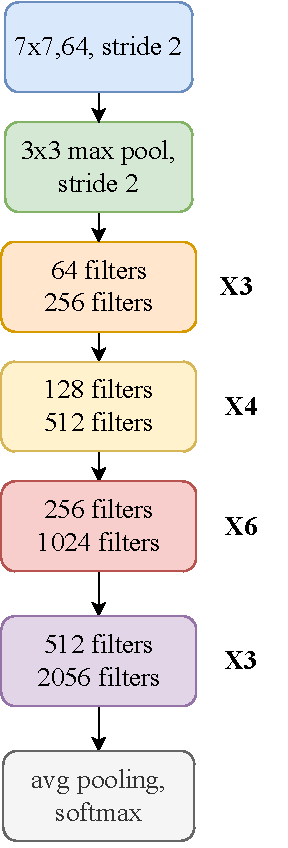
\includegraphics[scale=0.5]{arch-resnet}
		\caption{}
		\label{fig:resnet}
	\end{subfigure}
	\begin{subfigure}{0.4\textwidth}
		\centering
		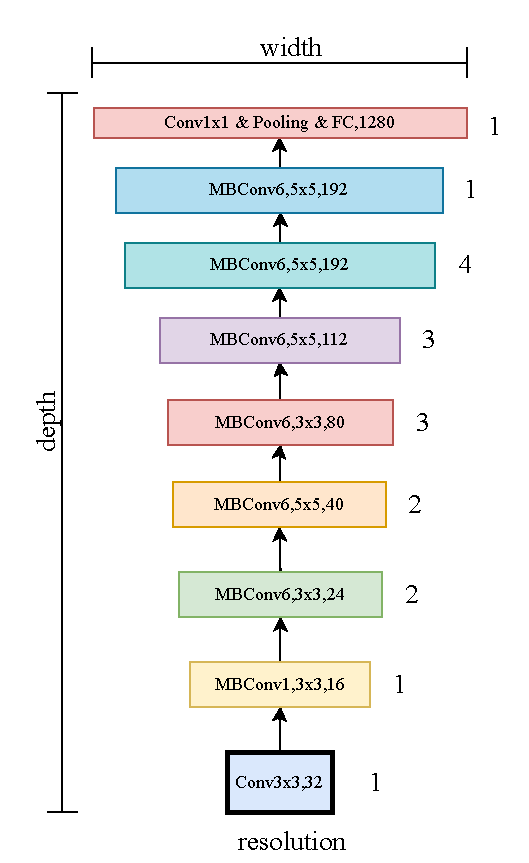
\includegraphics[scale=0.5]{arch-efficientnet}
		\caption{}
		\label{fig:efficientnet}
	\end{subfigure}
	\caption{Structures of ResNet50 and EfficientNet-B0. (a) ResNet 50 is composed of groups
			of residual blocks, each of which shares the same settings. The ``X'' besides the 
			block indicates the amount of residual blocks in that group. The numbers of filters
			inside indicates the filters used in the first two layers and output layer, respectively.
	(b) The EfficientNet models scale network width, depth, and resolution by a 
	factor $\phi$ to maintain a more balanced network. These factors are not
	independent to performance as we deal with more complex inputs. 
	Each stage includes the kernel size and filter count; the number besides
	each stage indicates the number of layers.}
	\label{fig:architectures}
\end{figure*}

\begin{table}
\centering
	\begin{tabular}{|c|c|c|}
		\hline
		& Parameters (Millions) & FLOPs (Billions) \\ \hline
			ResNet & 43.590 & 6.330 \\ \hline
			EfficientNetB3 & 11.483 & 0.274\\ \hline
	\end{tabular}

	\caption{Parameters and FLOPs of the two models tested. Although these might be slightly
	different than presented in their papers, they are quite similar. EfficientNet has much less
	parameters and FLOPs than an equivalent ResNet.}
	\label{tab:params}
\end{table}

\section{ArcFace}
ArcFace~\cite{Deng_2019_CVPR} tries to address some of the limitations of the commonly used
softmax loss in classification problems.

\begin{equation}
		L_1 = -\frac{1}{N}\sum_{i=1}^{n}\log\frac{e^{W^T_{yi}x_i + b_i}}{\sum_{j=1}^{n}e^{W^T_j x_i + b_j}}
\end{equation}

The authors claim that softmax does not provide higher intra-class similarity and lower inter-class samples.
In face recognition and verification, this means that the softmax cannot handle well differences in 
pose, angle or other such conditions for the same face.
Their proposed loss uses $l_2$ normalization on the weight matrix $W$  and the
input $x_i$.a
Then they multiply it by the cosine of the angle between $W$ and $x_i$.
With these changes, the embeddings are distributed on a hypershpere with a constant radios $s$
depending on the normalization.
Since all the outputs are now on a hypershpere, they introduce a margin penalty $m$
to improve intra-class compactness and inter-class discrepancy.
Their final loss is
\begin{equation}
		\mathbb{L} = -\frac{1}{N}\sum_{i=1}^{N}\log\frac{e^{s(\cos(\theta_{y_i}+m))}}{e^{s(\cos(\theta_{y_i} + m))} + \sum_{j=1, j\neq y_i}^{n}e^{s\cos(\theta_j)}}
\end{equation}

\section{Experiments}
For our experiments, we wanted to determine if changing the backbone has a significant impact on the accuracy.
The ArcFace paper uses a ResNet50 trained on the MS1MV3 dataset.
The authors released a model pretrained on this dataset which we also use in comparison.
To replace the lack of the original dataset, we use the CASIA-WebFace~\cite{casiawebface} dataset which 
contains 494,414 images collected from 10,575 different people.

For training, we have a ratio $r$ which indicates how many images of each identity we should use.
We tested $r=0.1, 0.25, 0.5, 1.0$.
This means that if a person has $10$ images in the dataset, using $r=0.1$ we train with $10*0.1 = 1$ images of that person.
We train each of our models for 12 epochs using a dynamic learning rate.
For data augmentations, we use \texttt{RandomHorizontalFlip()}, \texttt{CenterCrop((112, 112))}, and
normalizing the image.

In testing, our task becomes taking two images $x_1$ and $x_2$, and deterimining whether they 
contain the same person.
We would also like to test the low-light performance of our model.
For both test images, we apply the transformation
\[x_i = \sqrt{x_i} \times 2\]
and then cast $x_i$ into 8-bit unsigned integers.

For our results, we measured the precision-recall curves and ROC curves.
We tested the models we were able to train successfully and the baseline models.
The results are shown in~\ref{fig:pr} and~\ref{fig:roc}.

When using EfficientNet, the precision-recall and ROC curves all seem quite similar, near the 
baseline.
ResNet50 performs much better in the pr curve when using $r=0.25$, and slightly less better when
$r=.1$.
We did not train the model with $r=0.5$ due to time constraints.
\begin{figure*}
	\centering
	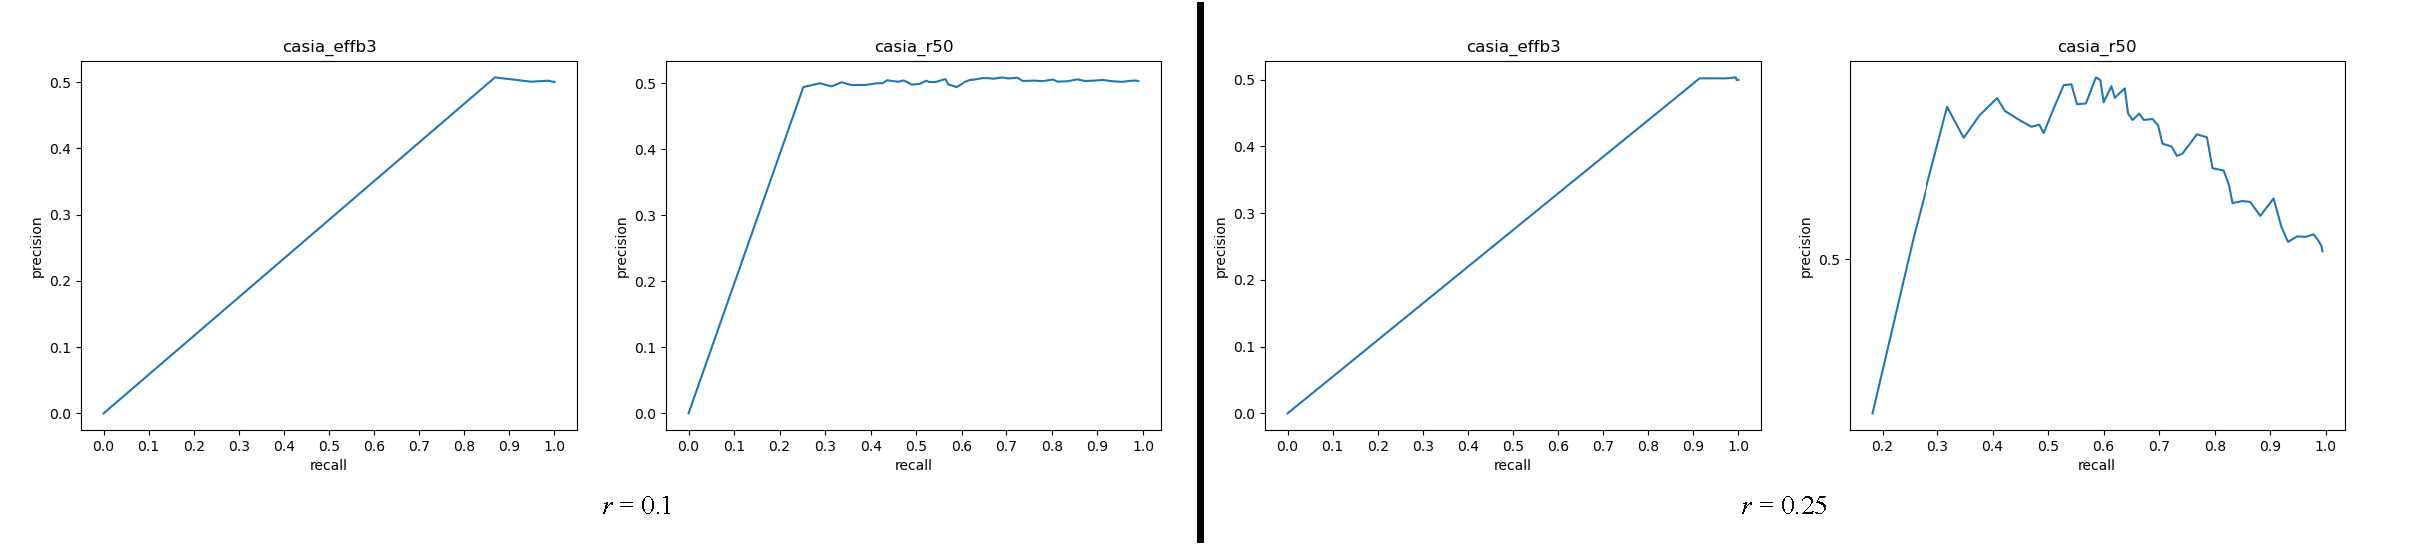
\includegraphics[scale=0.4]{pr_curves}
	\caption{Precision-Recall curves with 10\% and 25\% of the training data.}
	\label{fig:pr}
\end{figure*}
\begin{figure*}
	\centering
	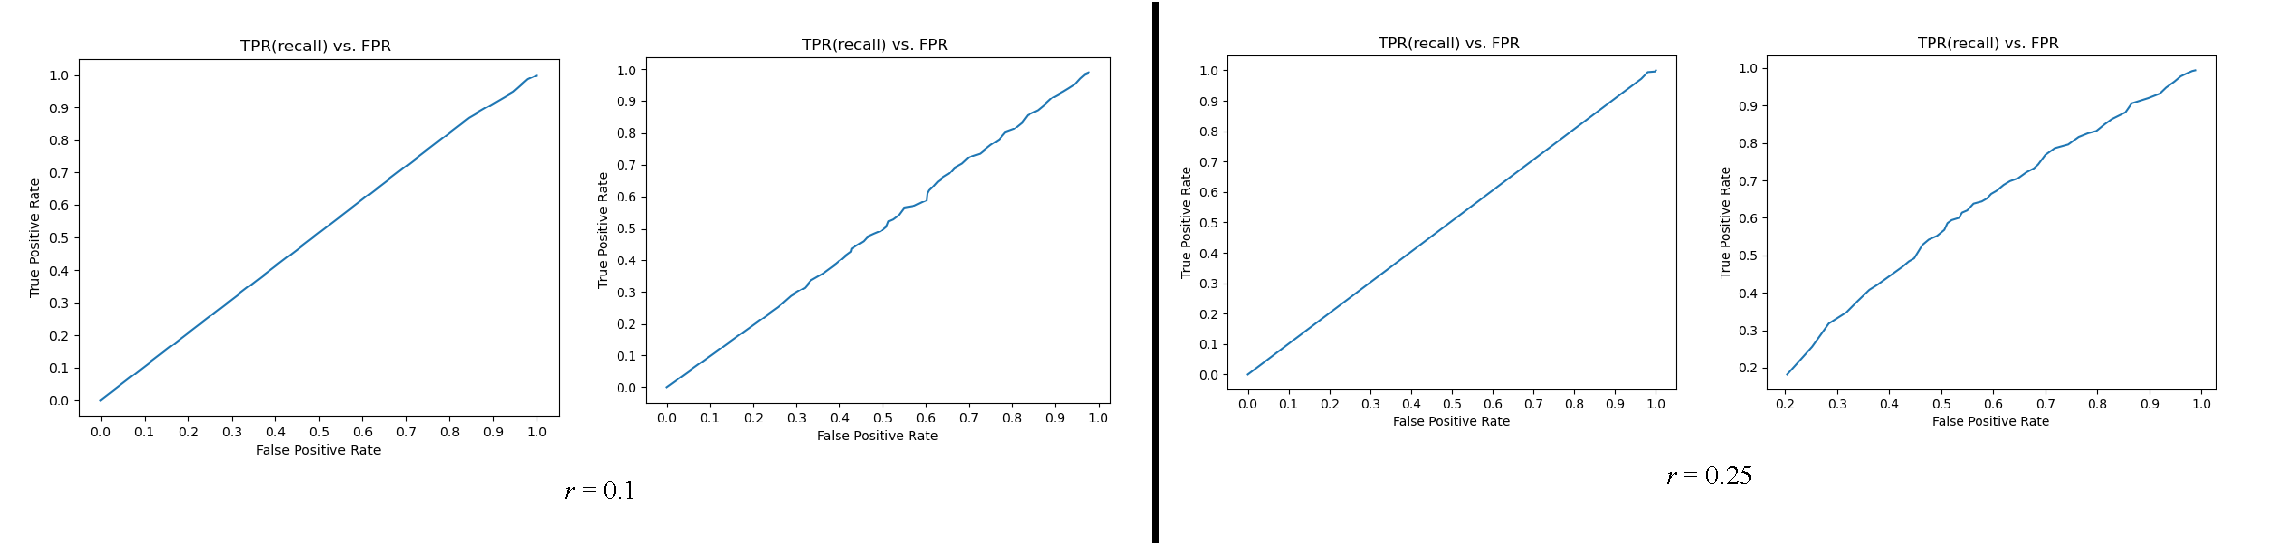
\includegraphics[scale=0.4]{roc_curves}
	\caption{ROC curves when using 10\% and 25\% of the training data.}
	\label{fig:roc}
\end{figure*}

We think that the reason the results are low compared to those in the paper due to the training regimen.
We were unable to access the labels they used to train their model.
While using the same hyperparameters for our model than the authors used, our verification accuracies
are still much lower.
Figures~\ref{fig:pre_trained_pr} and~\ref{fig:pre_trained_roc} show the precision-recall and ROC curves 
for the pre-trained model released by the authors and trained on the entire data set.


\begin{figure*}
	\centering
	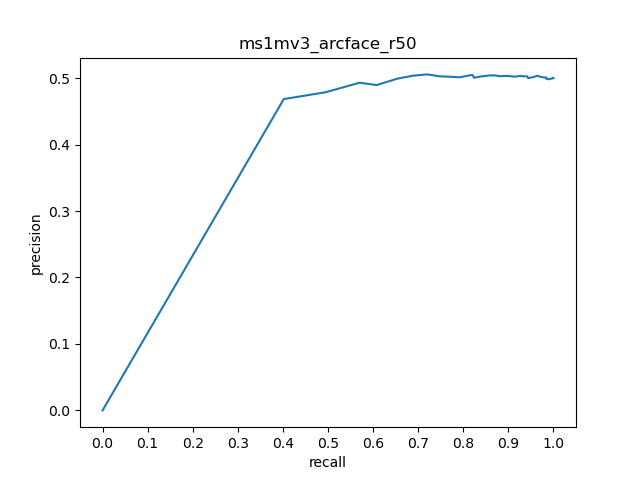
\includegraphics[scale=0.4]{ms1mv3_arcface_r50_pr}
	\caption{Precision recall curve on the pre-trained model released by authors. 
	The model was trained on ms1mv3, which was no longer available for download.}
	\label{fig:pre_trained_pr}
\end{figure*}
\begin{figure*}
	\centering
	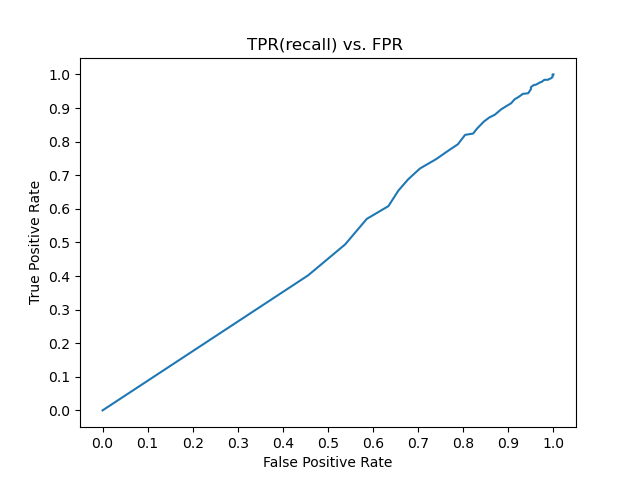
\includegraphics[scale=0.4]{ms1mv3_arcface_r50_roc}
	\caption{ROC curve on the pre-trained model released by authors. 
	The model was trained on ms1mv3, which was no longer available for download.}
	\label{fig:pre_trained_roc}
\end{figure*}

\section{Conclusions}
In conclusion, face verification is an important problem for computer vision, and requires different
methods than regular image classification.
We took the ArcFace method and tested the effect of using another baseline.
Although the results are low compared to the results in the paper, pre-trained models also struggled to 
achieve the performance shown in the paper.
However, without the specific evaluation script used by the authors it should not be surprising that the results
are different.

The EfficientNet model has much fewer parameters than ResNet yet is not used as much in the field.
Our goal was to show that these models can perform similarly while using much different amounts of parameters
and calculations.
\printbibliography
\end{document}
